%!TEX root = ../thesis_phd.tex
%%%%%%%%%%%%%%%%%%%%%%%%%%%%%%%%%%%%%%%%%%%%%%%%%%%%%%%%%%%%%%%%%%%%%%%%%%%%%%%%
% reconstruction.tex:
%%%%%%%%%%%%%%%%%%%%%%%%%%%%%%%%%%%%%%%%%%%%%%%%%%%%%%%%%%%%%%%%%%%%%%%%%%%%%%%%
\chapter{Event Reconstruction}
\label{reconstruction_chapter}
%%%%%%%%%%%%%%%%%%%%%%%%%%%%%%%%%%%%%%%%%%%%%%%%%%%%%%%%%%%%%%%%%%%%%%%%%%%%%%%%

In order to extract useful physics information from the \nova detector, the raw
data (cell hits) must be processed into higher level forms.
This processing step is known as reconstruction.
For this analysis, the primary goals of reconstruction are to identify \numu
charged-current (CC) interactions and estimate the energy of the neutrinos involved in the interactions. Identification of \numu CC interactions is really
a task of rejecting backgrounds induced by both cosmic rays and the \numi beam.  The cosmic ray background dominantly composed of down-going muons,
although other particles can also be present.  Backgrounds in the \numi beam
include both neutral current (NC) interactions and CC interactions from \nue or
\nutau.

Traditional reconstruction efforts involve detection of lines and other shapes
in raw data.  Classification is then a process of extracting manually
engineered features from those events which discriminate between signal and
background.
This analysis uses machine learned features in a convolutional neural network
to replace manual feature engineering.
The approach presented here differs in that the hits themselves are presented
to the neural network as two separate images, corresponding to $x$ (vertical)
and $y$ (horizontal) views.
The goal with this approach is to sidestep pathological failures incurred in each reconstruction and feature engineering step, thus allowing more of those pathological events to be more correctly classified.

The \nova \textit{event display} provides a visualization of the raw detector readout which serves as the input to reconstruction.
An example event display is shown in figure \ref{eventDisplay14}.
The data corresponds to 550 $\mu s$ of Far Detector (FD) readout, with hits colored according to their time recorded relative to the start of the readout window.
Visible activity displayed falls into two primary groups: randomly distributed electronic noise and correlated activity from cosmic rays.
Since cosmic rays cross the detector quickly, hits along each track are displayed as a uniform color.

\begin{figure}[t]
\begin{center}
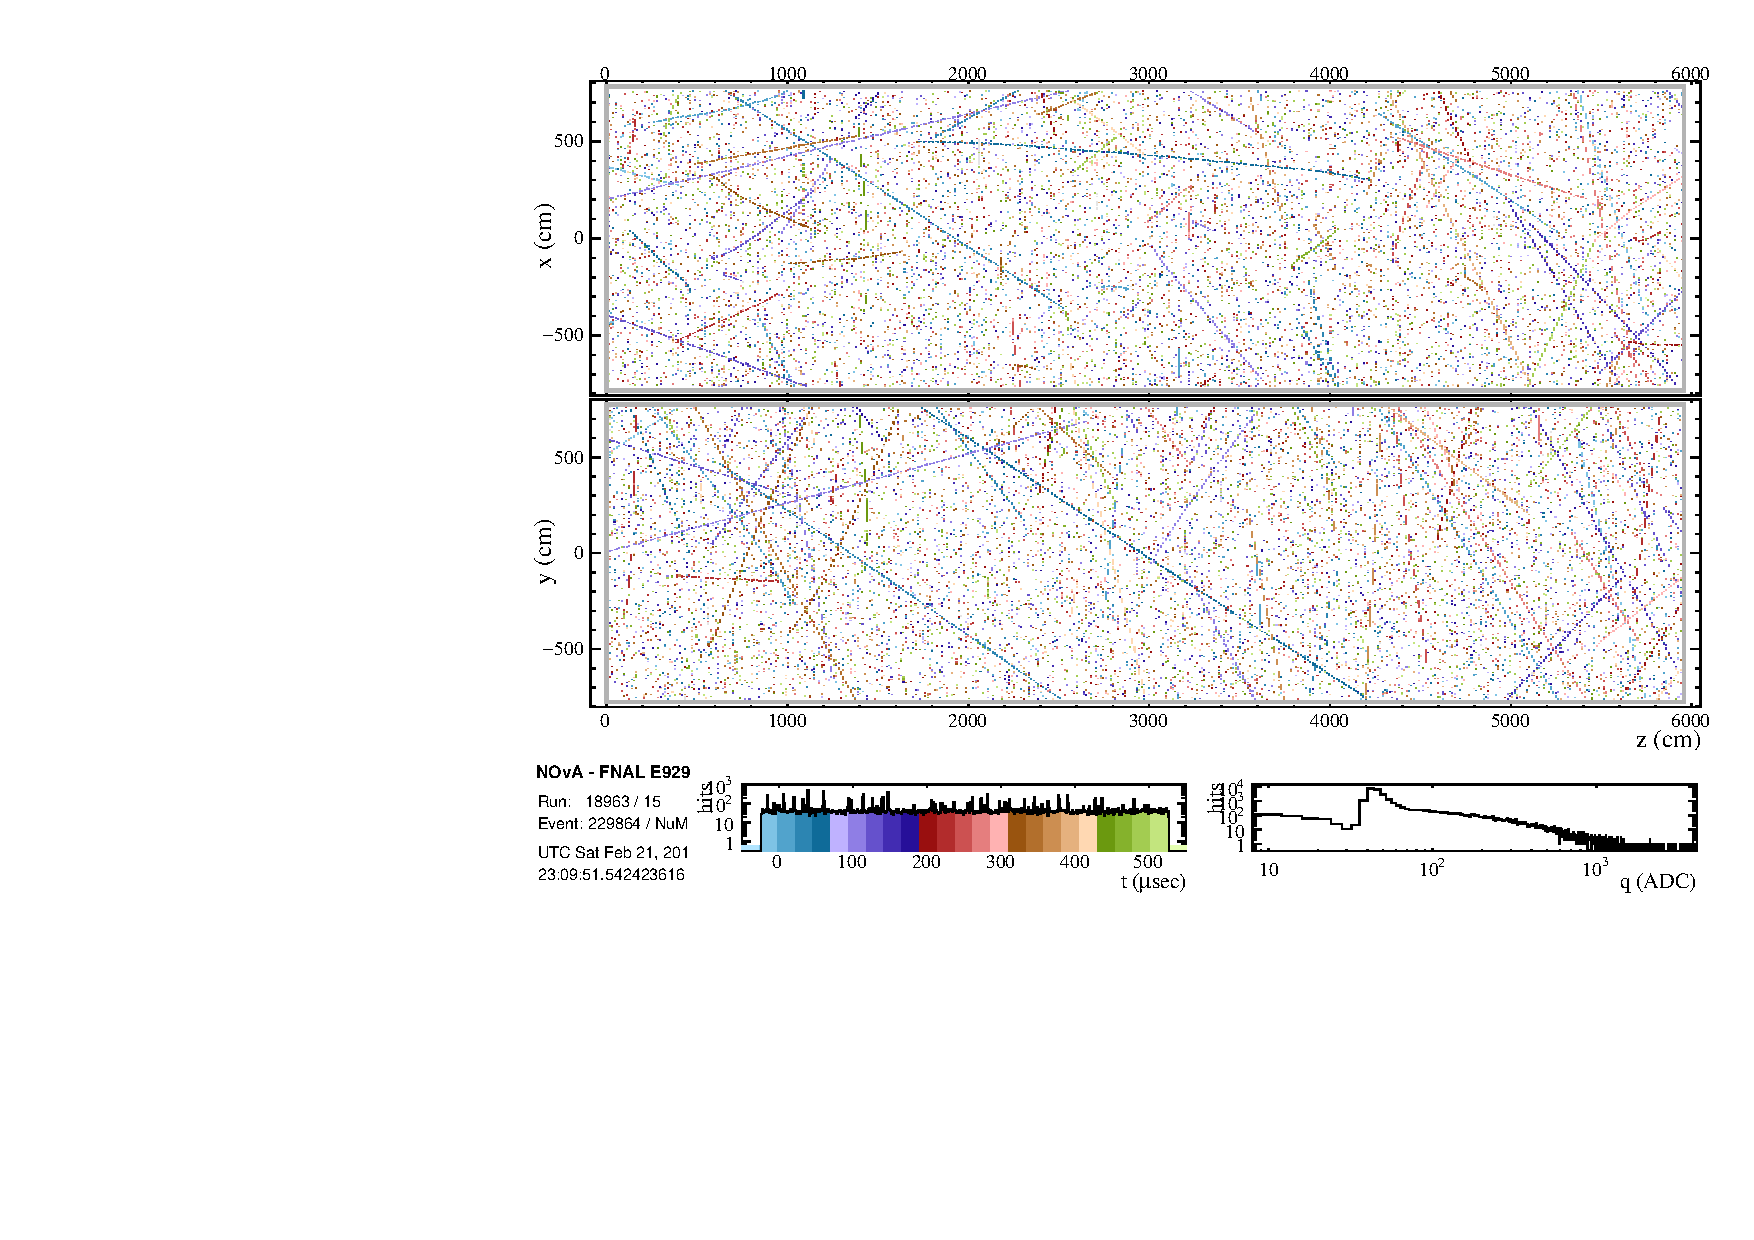
\includegraphics[width=\textwidth]{figures/evd/evd_14db.pdf}
\end{center}
\caption{An example \nova event display.  The top projection is an $x$ vs. $z$ view, the bottom is $y$ vs. $z$.  Hits are colored by the at which they were recorded relative to the start of the readout window; the color scale is visible in the bottom center pane.}
\label{eventDisplay14}
\end{figure}

\section{Slicing}

Reconstructing events in \nova first requires resolving activity within the
continuous readout windows.
In other words, the continuous readout of noise and physics activity must be
separated into groups of hits which correspond to individual particle
interactions.
This task is referred to as \textit{slicing}.

\begin{figure}[t]
\begin{center}
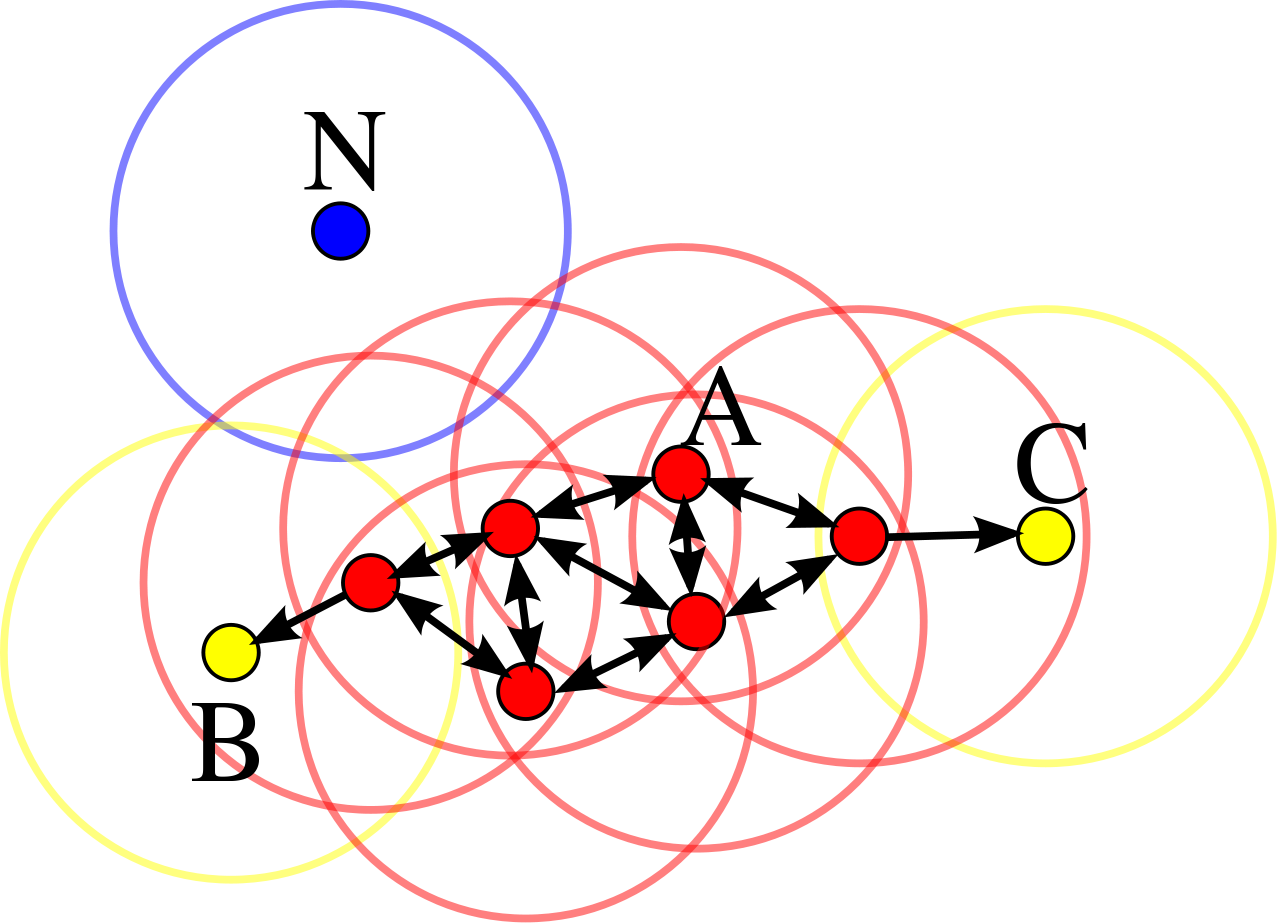
\includegraphics[width=0.7\textwidth]{figures/figures/dbscan.png}
\end{center}
\caption{Depiction of clustering with the DBSCAN algorithm.}{Depiction of
clustering with the DBSCAN algorithm.
The open circles around each point are drawn with a radius to represent the
neighbor distance threshold.
The red points, for instance point A, are
considered to be \textit{core} points since they have as many or more neighbors
than the minimum required to form a cluster.  The yellow points, including B
and C, are called
\textit{edge} points since they have fewer neighbors than the minimum required
to make a cluster, but included in the cluster with the red points since they
are below the neighbor distance threshold.  The blue point is not part of the
cluster since its distance from all other points exceeds the neighbor threshold.
}
\label{dbscan}
\end{figure}

Slicing in \nova is achieved through an implementation of the DBSCAN algorithm
\cite{ester1996density}.
The algorithm evaluates the distance between every pair of points based on
a distance metric which suits the problem at hand.
If the distance between a pair of points is below a threshold, $\epsilon$, the
points are added to the same cluster.
Clusters can be disregarded if they do not inude a minimum number of hits,
which can be optimized based on the amount of noise in the data.
A depiction of how points are clustered can be seen in figure \ref{dbscan}.

The distance metric used for slicing in \nova is based on the time, $t$, and
spatial position, $\vec{r}$, of hits
\begin{equation}
L = \bigg( \frac{\Delta t - \Delta \vec{r} / c }{T} \bigg)^2 +
     \bigg( \frac{\Delta \vec{r}}{D} \bigg)^2,
\end{equation}

where $c$ is the speed of light.  The parameters $T$ and $D$ are configurable
length scales which dictate the relative weight of separation in time and
space.

The slicing algorithm for \nova has been tuned such that it provides good
separation between cosmic rays while leaving entire neutrino interactions
in tact.  Certain delayed activity, such as Michel electrons (from muon decay)
and neutron activity is prone to being excluded from a slice.
Generally, however, a slice in \nova data is treated as a potential cosmic ray
or entire neutrino interaction with all daughter particles.


\section{Tracking}

Once particle interactions have been resolvde

\subsection{Least-squares Regression}

We fit lines to regions of tracks.


\subsection{Kalman Filtering}

We expand tracks from pairs based on chi-square.

\section{Calibration}

An important input to many reconstruction efforts is an accurate estimate of
the energy deposited in a cell.  Calibration procedures aim provide an the
estimation of energy deposition based on the recorded ADC value and position
of a particular cell hit.  The \nova calibration accounts for three primary
effects: attenuation
of light in the wavelength shifting fiber, cell-to-cell variations, and
conversion conversion from ADC scale to physical energy units.

\subsection{Attenuaiton and Cell-to-cell Corerection}

The attenuation correction is based upon cosmic ray muons since they are
abundant and their energy deposition properties are well understood.  A
reference sample of cell hits is selected from muon tracks which satisfy a few
simple characteristics.  First, tracks must touch two detector faces,
indicating that they traversed the detector rather than stopping inside.  The
tracks are required to cross at least ten planes to ensure that path length
(distance traversed by the muon within each cell) can accurately be estimated.
Hits on selected tracks are only used for calibration if they satisfy the
so-called tri-cell criterion; that is, that there are also hits present in
adjacent planes.  This criterion also helps ensure that a reasonable path
length estimate is obtained.  Certain cells fail to produce enough its to allow
the subsequent attenuation fits to be obtained, for instance cells on the edges
of the detector and those adjacent to dead cells.  Such cells are calibrated
with alternative samples with hits in adjacent cells.


\begin{figure}[t]
\begin{center}
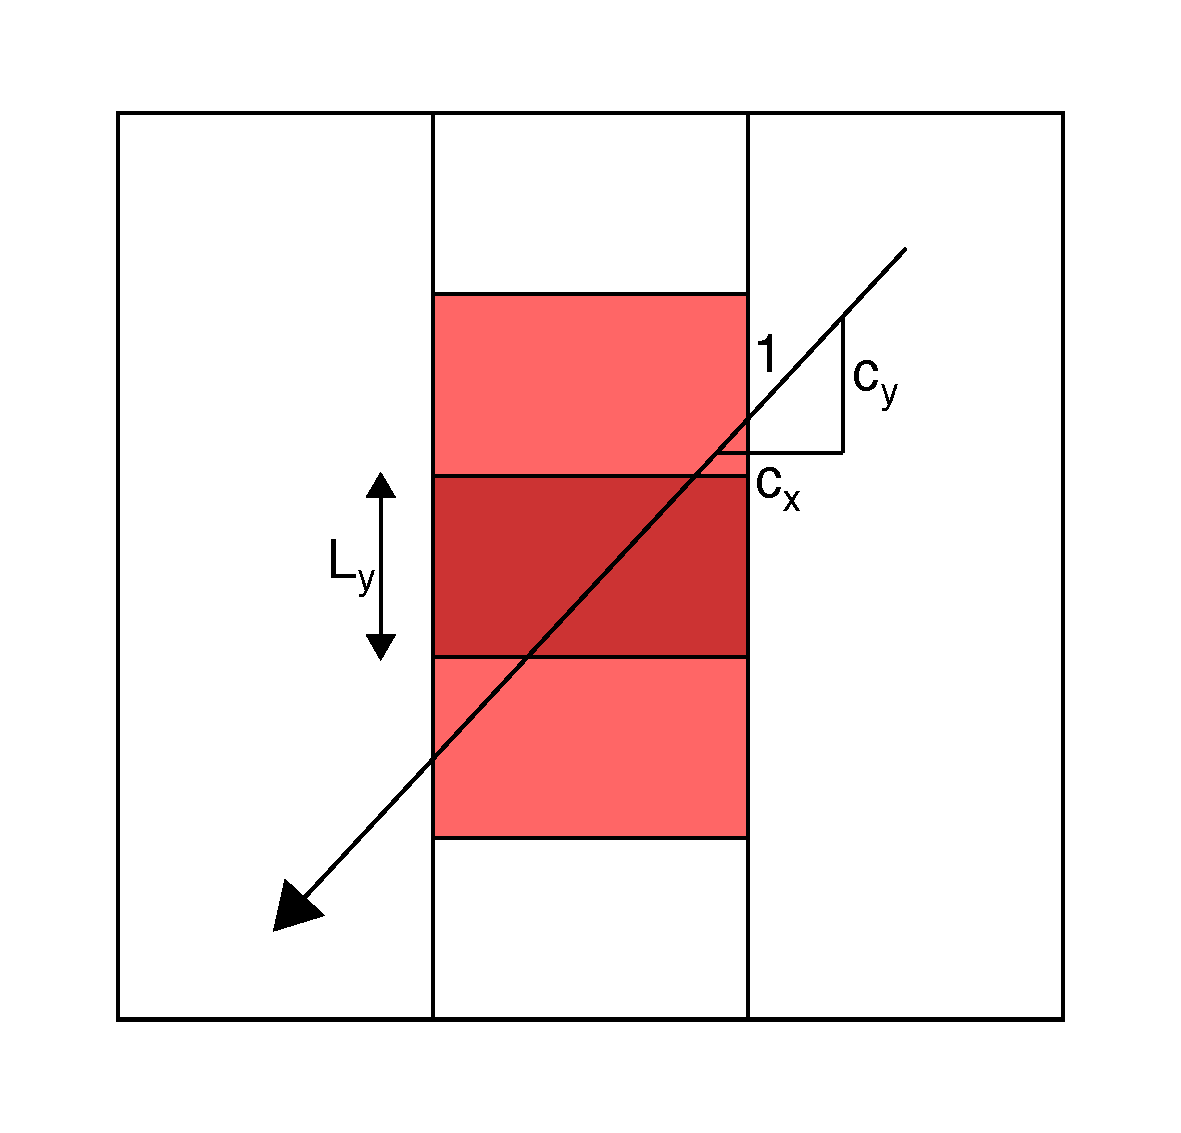
\includegraphics[width=0.8\textwidth]{figures/plots/reco/calib_tricell}
\end{center}
\caption{Depiction of a tri-cell hit used for calibration.  The precence of
activity in the two adjacent cells helps ensure an accurate estimate of
path length traversed by a muon through a cell.}
\label{calib_tricell}
\end{figure}

For each reference hit, the ADC value is converted to PE based on a scale
factor.  The path length and position along the cell (i.e. distance from the
APD readout) are both estimated from the muon track trajectory.
A 2D histogram of the ratio of PE to path length vs. position along cell is
constructed for each cell.
A fit is to the mean PE per path length response function of
position is used to characterize each cell.
The functional form for the middle part of the cells is a sum of two
exponentials, one corresponding the short trip to the APD and the other for
the long way to the far end of the cell and back around the fiber loop.
\begin{equation}
y(W) = C + \bigg ( \exp \big( \frac{W}{X}\big) +
\exp \big( - \frac{L + W}{X}\big)  \bigg )
\end{equation}
Above, $W$ is the position along the cell, $X$ is the fiber attenuation length,
and $L$ is the length of the cell.
The attenuation length as well as constants $C$ and $A$ are free parameters
in the fit.
At the end of cells, a diminished response known as \textit{roll-off} has been
observed, presumedly due
to light being absorbed at the ends rather than in the fiber.
The deficit of light is empirically well described by an $x^4$ form
\begin{equation}
  y=\left\{\begin{tabular}{cl}
    $1-\alpha_R(x-x_R)^4$ & $x>+x_R$\\
    1 & otherwise\\
    $1-\alpha_L(x-x_L)^4$ & $x<-x_L$
  \end{tabular}\right.
  \label{eqn:rolloffs}
\end{equation}
where free parameters $x_R$ and $x_L$ indicate the start of the roll-off
region on either side and $\alpha_R, \alpha_L$  determine the scale.
These fits are often not robust, however, so they are not used.
Alternatively, an interpolation method called LOWESS \cite{cleveland1981lowess}
is used to correct the residuals from the exponential form.
In addition to picking up the roll-off behavior, the LOWESS fits also serve to
correct other significant deviations observed in the data far from the ends of
the cells.
These deviations are believed to be caused by any peculiar positioning of the
fiber within a cell which could affect light collection.
The curve produced by LOWESS at any point is the weighted mean of the
deviations,
\begin{equation}
  w_i=\left(1-\left|{x-x_i\over\sigma}\right|^3\right)^3
\end{equation}
where the smoothing length scale $\sigma$ is 30cm.
Examples of the final fits with LOWESS corrections can be seen in figure
\ref{calib_atten}.

\begin{figure*}
  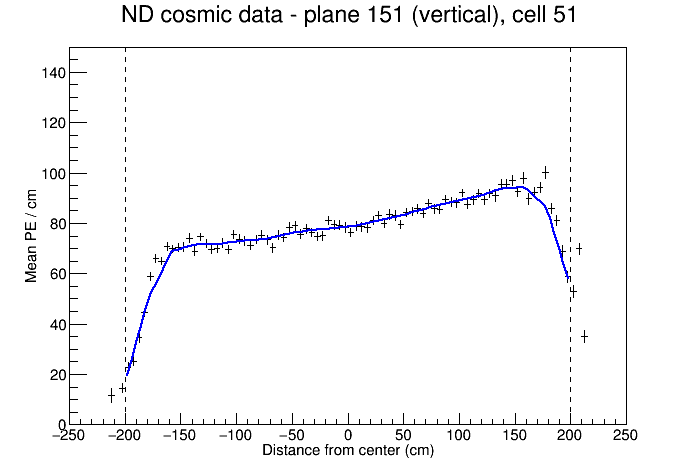
\includegraphics[width=.5\linewidth]{figures/plots/reco/calib_totfit_data_inX_151_051}
  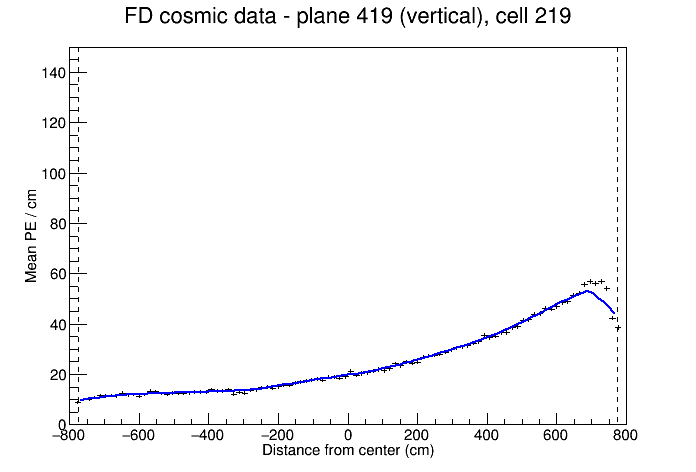
\includegraphics[width=.5\linewidth]{figures/plots/reco/calib_totfit_data_inX_419_219}
  \caption[]{Example of a good Near (left) and Far (right) detector fit,
  showing attenuation fits with LOWESS corrections.}\label{calib_atten}
\end{figure*}

The attenuation fits determine the mean response to cosmic ray muons is
can be determined for a hit at any position in the detector.
Thus, the calibrated response for any hit is the ratio of its PE to result of
the fit at that position.  At this point, the energy in absolute units is
still unknown, but the effects of attenuation and cell-by-cell variations
have been mitigated.

\subsection{Absolute Energy Calibration}

The absolute energy calibration is responsible for converting the corrected
PE value described in the previous section into a value which corresponds
to meaningful physical units.
Muon tracks which stop inside the detector form a reference sample with well
understood energy deposition characteristics.
Near the end of particle tracks, the energy deposition per unit length
(\dedx) is well described by the Bethe-Bloch formula \cite{pdg}.
The formula predicts a stable minimum in \dedx near the track end,
which for muons in organic materials covers a wide range of several hundred cm.
This stable region is demonstrated in figure \ref{calib_dEdX}.
For \nova, the region between 100 and 200 cm from the track endpoint is used
to determine the absolute energy scale.

\begin{figure}[t]
\begin{center}
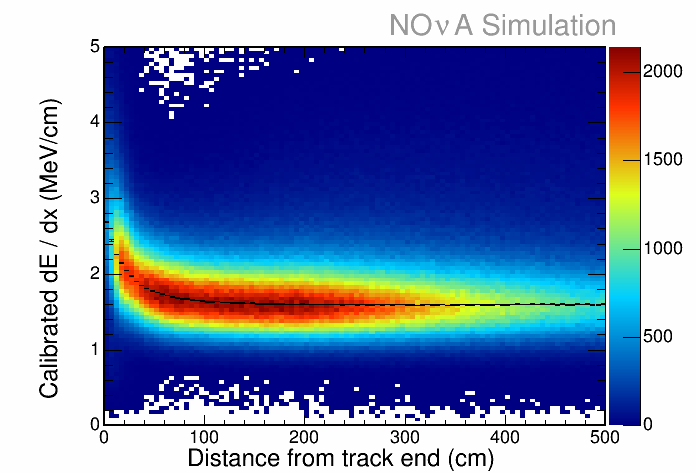
\includegraphics[width=0.8\textwidth]{figures/plots/reco/calib_dEdX.png}
\end{center}
\caption{2D histogram depicting deposited energy per path length (dE/dX) for
cell hits after attenuation and cell-to-cell correction.  The color scale
indicates the number of measurements in each bin.  The rise in energy at the
end of muon track (left) is well described by the Bethe-Bloch formula \cite{pdg}.}
\label{calib_dEdX}
\end{figure}

\section{Image Formation}

\section{Architecture and Training}

We use siamese googlenet, two googlenets side-by-side

Train on neutrinos, then add cosmics and fine tune.




%%%%%%%%%%%%%%%%%%%%%%%%%%%%%%%%%%%%%%%%%%%%%%%%%%%%%%%%%%%%%%%%%%%%%%%%%%%%%%%%
